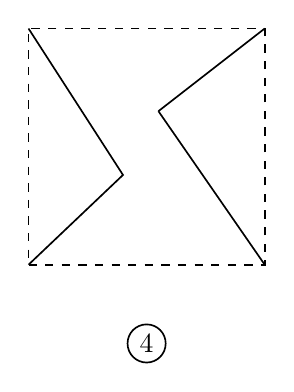
\begin{tikzpicture}[x=1cm,y=1cm,font=\normalsize,
 geometry edge/.style={solid,line width=.6pt},
 geometry mark/.style={solid,line width=.6pt},
 geometry label/.style={font=\normalsize,inner sep=2pt}]
\coordinate (S3) at (0,0);
\coordinate (S2) at (3,0);
\coordinate (S1) at (3,3);
\coordinate (S0) at (0,3);
\coordinate (M1) at (1.2,1.14);
\coordinate (M2) at (1.65,1.95);
\draw[geometry edge,dashed] (S3)--(S2)--(S1)--(S0)--cycle;
\draw[geometry edge] (S0)--(M1)--(S3);
\draw[geometry edge] (M2)--(S1);
\draw[geometry edge] (M2)--(S2);
\node[draw,circle,line width=.6pt,inner sep=2pt,font=\normalsize] at (1.5,-1.0) {4};
\end{tikzpicture}
